\item \points{35} {\bf Implicit Regularization}

Recall that in the overparameterized regime (where the number of parameters is larger than the number of samples), typically there are infinitely many solutions that can fit the training dataset perfectly, and many of them cannot generalize well (that is, they have large test errors). However, in many cases, the particular optimizer we use (e.g., GD, stochastic GD with particular learning rates (see part (g) for more details), batch sizes, noise, etc.) tends to find solutions that generalize well. This phenomenon is called implicit regularization effect (also known as algorithmic regularization or implicit bias). 

In this problem, we will look at the implicit regularization effect on two toy examples in the overparameterized regime: linear regression and a quadratically parameterized model. For linear regression, we will show that gradient descent with zero initialization will always find the minimum norm solution (instead of an arbitrary solution that fits the training data), and in practice, the minimum norm solution tends to generalize well. For a quadratically parameterized model, we will show that initialization and batch size also affect generalization.

\begin{enumerate}
    \item\subquestionpoints{3} Suppose we have a dataset $\{(x^{(i)}, y^{(i)});i=1,\cdots,n\}$ where $x^{(i)}\in \R^{d}$ and $y^{(i)}\in \R$ for all $1\le i\le n.$ We assume the dataset is generated by a linear model without noise. That is, there is a vector $\beta^\star\in\R^{d}$ such that $y^{(i)}=(\beta^\star)^\top x^{(i)}$ for all $1\le i\le n$. Let $X\in \R^{n\times d}$ be the matrix representing the inputs (i.e., the $i$-th row of $X$ corresponds to $x^{(i)})$) and $\vec{y}\in\R^{n}$ the vector representing the labels (i.e., the $i$-th row of $\vec{y}$ corresponds to $y^{(i)})$):
$$
	X=
\begin{bmatrix}
	- & x^{(1)} & - \\
	- & x^{(2)} & - \\
	\vdots & \vdots & \vdots\\
	- & x^{(n)} & - 
\end{bmatrix},\qquad
\vec{y}=
\begin{bmatrix}
y^{(1)} \\
y^{(2)}\\
\vdots\\
y^{(n)}
\end{bmatrix}.
$$
Then in matrix form, we can write $\vec{y}=X\beta^\star.$
We assume that the number of examples is less than the number of parameters (that is, $n<d$).

We use the least-squares cost function to train a linear model:
\begin{equation}\label{equ:mse}
	J(\beta)=\frac{1}{2n}\|X\beta-\vec{y}\|_2^2.
\end{equation}

In this sub-question, we characterize the family of global minimizers to Eq.~\eqref{equ:mse}. We assume that $X X^\top\in \R^{n\times n}$ is an invertible matrix. \textbf{Prove that} $\beta$ achieves zero cost in Eq.~\eqref{equ:mse} if and only if 
\begin{equation}\label{equ:ir2}
	\beta=X^\top (XX^\top)^{-1}\vec{y}+\zeta
\end{equation} for some $\zeta$ in the subspace orthogonal to all the data (that is, for some $\zeta$ such that $\zeta^\top x^{(i)}=0,\forall 1\le i\le n.$) 

Note that this implies that there is an infinite number of $\beta$'s such that Eq.~\eqref{equ:mse} is minimized. We also note that $X^\top (XX^\top)^{-1}$ is the pseudo-inverse of $X$, but you don't necessarily need this fact for the proof.


    	\ifnum\solutions=1 {
	\begin{answer}
\newpage
\end{answer}

    	}\fi
    
    
    \item\subquestionpoints{3} We still work with the setup of part (a). Among the infinitely many optimal solutions of Eq.~\eqref{equ:mse}, we consider the \textit{minimum norm} solution. Let $\rho=X^\top (X X^\top)^{-1}\vec{y}$. In the setting of (a), \textbf{prove that} for any $\beta$ such that $J(\beta)=0$, $\|\rho\|_2\le \|\beta\|_2.$ In other words, $\rho$ is the minimum norm solution.

\emph{Hint:} As a intermediate step, you can prove that for any $\beta$ in the form of Eq.~\eqref{equ:ir2}, $$\|\beta\|_2^2=\|\rho\|_2^2+\|\zeta\|_2^2.$$
    \ifnum\solutions=1 {
    	\begin{answer}
\newpage
\end{answer}
    	}\fi
    
    \item\subquestionpoints{5} 
\textbf{Coding question: minimum norm solution generalizes well}

For this sub-question, we still work with the setup of parts (a) and (b). We use the following datasets:
\begin{center}
	\url{src/implicitreg/ir1_train.csv, ir1_test.csv}
\end{center}
Each file contains $d+1$ columns. The first $d$ columns in the $i$-th row represents $x^{(i)}$, and the last column represents $y^{(i)}.$ In this sub-question, we use $d=200$ and $n=40$.

Using the formula in sub-question (b), \textbf{compute} the minimum norm solution using the training dataset. Then, \textbf{generate} three other different solutions with zero costs and different norms using the formula in sub-question (a).
The starter code is in \url{src/implicitreg/linear.py}. \textbf{Plot} the test error of these solutions (including the minimum norm solution) in a scatter plot. 
Use the norm of the solutions as $x$-axis, and the test error as $y$-axis. For your convenience, the plotting function is provided as the method \url{generate_plot} in the starter code. 
Your plot is expected to demonstrate that the minimum norm solution generalizes well.
	\ifnum\solutions=1 {
		
\begin{answer}
\begin{figure}[H]
    \centering
    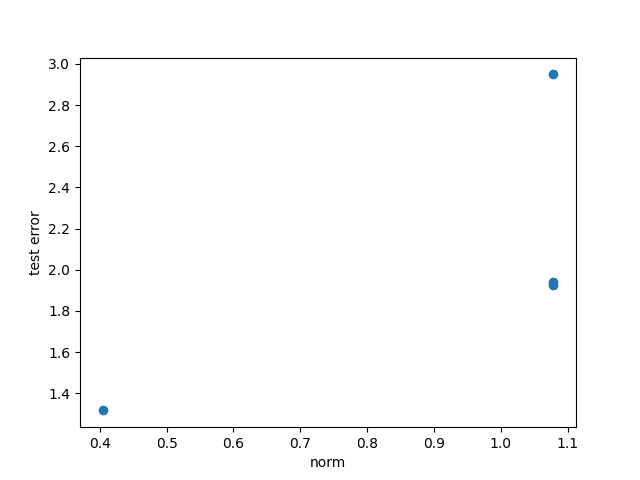
\includegraphics[width=9cm]{implicitreg/implicitreg_linear.png}
\end{figure}
From the plot, we observe that the solution with the minimum norm, $\rho$ has lower test error among the solution. That is in line with the hypothesis that the minimum norm solution should generalize well.
The other solutions were obtained by taking random vectors from the nullspace of $X$ and adding them to the min-norm solution.
\end{answer}
		}\fi
	
	\item\subquestionpoints{5} For this sub-question, we work with the setup of part (a) and (b). In this sub-question, you will prove that the gradient descent algorithm with \emph{zero initialization} always converges to the minimum norm solution. Let $\beta^{(t)}$ be the parameters found by the GD algorithm at time step $t$. Recall that at step $t$, the gradient descent algorithm update the parameters in the following way
\begin{equation}
	\beta^{(t)}=\beta^{(t-1)}-\eta\nabla J(\beta^{(t-1)})=\beta^{(t-1)}-\frac{\eta}{n} X^\top (X\beta^{(t-1)}-\vec{y}).
\end{equation}
As in sub-question (a), we also assume $X X^\top$ is an invertible matrix. \textbf{Prove} that if the GD algorithm  with zero initialization converges to a solution $\hat{\beta}$ satisfying $J(\hat{\beta})=0$, then $\hat{\beta}=X^\top(XX^\top)^{-1}\vec{y}=\rho$, that is, $\hat{\beta}$ is the minimum norm solution.

\emph{Hint:} As a first step, you can prove by induction that if we start with zero initialization, $\beta^{(t)}$ will always be a linear combination of $\{x^{(1)}, x^{(2)}, \cdots, x^{(n)}\}$ for any $t\ge 0.$ Then, for any $t\ge 0$, you can write $\beta^{(t)}=X^\top v^{(t)}$ for some $v^{(t)}\in \R^{n}.$ As a second step, you can prove that if $\hat{\beta}=X^\top v^{(t)}$ for some $v^{(t)}$ and $J(\hat{\beta})=0$, then we have $\hat{\beta}=\rho.$

You don't necessarily have to follow the steps in this hint. But if you use the hint, you need to prove the statements in the hint.

	\ifnum\solutions=1 {
		
\begin{answer}
\newpage
\end{answer}
	}\fi

	\item\subquestionpoints{3}
In the following sub-questions, we consider a slightly more complicated model called quadratically parameterized model. A quadratically parameterized model has two sets of parameters $\theta,\phi\in \R^{d}$. Given a $d$-dimensional input $x\in \R^{d}$, the output of the model is 
\begin{align}
	f_{\theta,\phi}(x)=\sum_{k=1}^{d}\theta_k^2 x_k - \sum_{k=1}^{d}\phi_k^2 x_k.\label{eqn:1}
\end{align}
Note that $f_{\theta,\phi}(x)$ is linear in its input $x$, but non-linear in its parameters $\theta,\phi.$ Thus, if the goal was to learn the function, one should simply just re-parameterize it with a linear model and use linear regression. However, here we insist on using the parameterization above in Eq.~\eqref{eqn:1} in order to study the implicit regularization effect in models that are nonlinear in the parameters.

\emph{Notations:} To simplify the equations, we define the following notations. For a vector $v\in \R^{d},$ let $v^{\odot 2}$ be its element-wise square (that is, $v^{\odot 2}$ is the vector $[v_1^2, v_2^2,\cdots, v_d^2]\in \R^{d}.$)  For two vectors $v,w\in \R^{d},$ let $v\odot w$ be their element-wise product (that is, $v\odot w$ is the vector $[v_1w_1,v_2w_2,\cdots,v_dw_d]\in \R^{d}.$) Then our model can be written as 
\begin{align}
	f_{\theta,\phi}(x)=x^\top (\theta^{\odot 2} -\phi^{\odot 2}).
\end{align}

Suppose we have a dataset $\{(x^{(i)}, y^{(i)});i=1,\cdots,n\}$ where $x^{(i)}\in \R^{d}$ and $y^{(i)}\in \R$ for all $1\le i\le n,$ and $$y^{(i)}=(x^{(i)})^\top ((\theta^\star)^{\odot 2}- (\phi^\star)^{\odot 2})$$ for some $\theta^\star, \phi^\star\in \R^{d}$.
Similarly, we use $X\in \R^{n\times d}$ and $\vec{y}\in \R^{n}$ to denote the matrix/vector representing the inputs/labels respectively:
$$
X=
\begin{bmatrix}
	- & x^{(1)} & - \\
	- & x^{(2)} & - \\
	\vdots & \vdots & \vdots\\
	- & x^{(n)} & - 
\end{bmatrix},\qquad
\vec{y}=
\begin{bmatrix}
	y^{(1)} \\
	y^{(2)}\\
	\vdots\\
	y^{(n)}
\end{bmatrix}.
$$
Let $J(\theta,\phi)=\frac{1}{4n}\sum_{i=1}^{n}(f_{\theta,\phi}(x^{(i)})-y^{(i)})^2$ be the cost function.

First, when $n<d$ and $XX^\top$ is invertible, \textbf{prove} that there exists infinitely many optimal solutions with zero cost.

\emph{Hint:} Find a mapping between the parameter $\beta$ in linear model and the parameter $\theta,\phi$ in quadratically parameterized model. Then use the conclusion in sub-question (a).
	\ifnum\solutions=1 {
		
\begin{answer}
\newpage
\end{answer}
	}\fi

	\item\subquestionpoints{10}\textbf{} \textbf{Coding question: implicit regularization of initialization}

We still work with the setup in part (e).
For this sub-question, we use the following datasets:
\begin{center}
	\url{src/implicitreg/ir2_train.csv, ir2_test.csv}
\end{center}
Each file contains $d+1$ columns. The first $d$ columns in the $i$-th row represents $x^{(i)}$, and the last column represents $y^{(i)}.$ In this sub-question, we use $d=200$ and $n=40$.

First of all, the gradient of the loss has the following form:
\begin{align}
	\nabla_\theta J(\theta,\phi)&=\frac{1}{n}\sum_{i=1}^{n}((x^{(i)})^\top (\theta^{\odot 2} -\phi^{\odot 2})-y^{(i)})(\theta\odot x^{(i)}),\\
	\nabla_\phi J(\theta,\phi)&=-\frac{1}{n}\sum_{i=1}^{n}((x^{(i)})^\top (\theta^{\odot 2} -\phi^{\odot 2})-y^{(i)})(\phi\odot x^{(i)}).
\end{align}
You don't need to prove these two equations. They can be verified directly using the chain rule.

Using the formula above, run gradient descent with initialization $\theta=\alpha \mathbf{1}, \phi=\alpha\mathbf{1}$ with $\alpha\in \{0.1, 0.03, 0.01\}$ (where $\mathbf{1}=[1,1,\cdots,1]\in\R^{d}$ is the all-1's vector) and learning rate $0.08$. We provide the starter code in \url{src/implicitreg/qp.py}. \textbf{Plot} the curve of training error and testing error with different $\alpha$. Use the number of gradient steps as $x$-axis, and training/testing error as $y$-axis. Include your plot in the writeup and \textbf{answer} the following two questions based on your plot: which models can fit the training set? Which initialization achieves the best test error? 

\textit{Remark:} Your plot is expected to demonstrate that the initialization plays an important role in the generalization performance---different initialization can lead to different global minimizers with different generalization performance. In other words, the initialization has an implicit regularization effect. 
	\ifnum\solutions=1 {
		
\begin{answer}
\newpage
\begin{figure}[H]
    \centering
    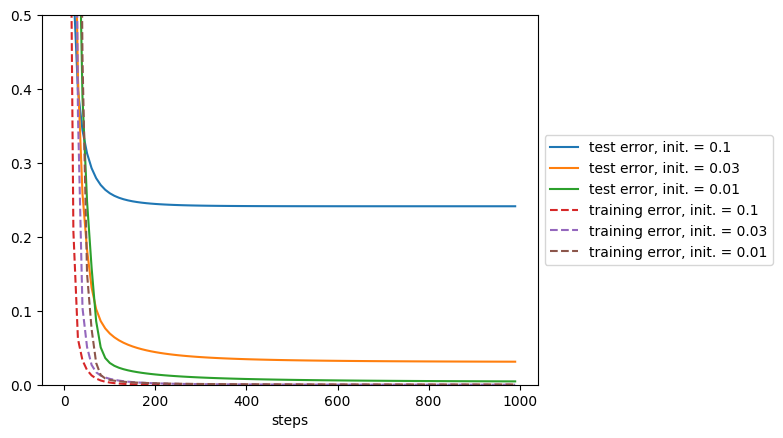
\includegraphics[width = 13cm]{implicitreg/implicitreg_quadratic_initialization.png}
\end{figure}
From the plot, we observe that all of the models can fit the training set. Howerver the perfomance on the test set is much better for init $0.01, 0.03$ than $0.1$. init 0.01 has the best test error.
\end{answer}
	}\fi

	\item\subquestionpoints{6}\textbf{} \textbf{Coding question: implicit regularization of batch size}

We still work with the setup in part (e). For this sub-question, we use the same dataset and starter code as in sub-question (f). We will show that introducing noise in the training process also induces implicit regularization. In particular, we will observe how noise introduced by \emph{stochastic} gradient descent (SGD) helps generalization. The gradient descent algorithm we have covered so far in lecture is also known as \emph{batch} gradient descent, in which we look at the entire training set before taking a single update step. In SGD, we only look at a subset of the training examples before taking an update step. (Note that ``true" SGD looks at a single training example before taking an update step. In this problem, we will also be considering the generalization of SGD -- mini-batch gradient descent -- to generate more empirical evidence for your final observation!) SGD will be covered in more detail later in the course, but this is all you need to know to solve this problem.

\textbf{Implement} the SGD algorithm, and \textbf{plot} the training and test errors with mini-batch sizes $\{1, 5, 40\}$, learning rate $0.08$, and initialization $\alpha=0.1$. Similarly, use the number of gradient steps as $x$-axis, and training/test error as $y$-axis. For simplicity, the code for selecting a batch of examples is already provided in the starter code.
\textbf{Compare} the results with those in sub-question (g) with the same initialization. Does SGD find a better solution?

Your plot is expected to show that the stochasticity in the training process is also an important factor in the generalization performance --- in our setting, SGD finds a solution that generalizes better. In fact, a conjecture is that stochasticity in the optimization process (such as the noise introduced by a small batch size) helps the optimizer to find a solution that generalizes better. This conjecture can be proved in some simplified cases, such as the quadratically parameterized model in this sub-question (adapted from the paper \href{https://arxiv.org/abs/2006.08680}{HaoChen et al., 2020}), and can be observed empirically in many other cases.
	\ifnum\solutions=1 {
		
\begin{answer}
\begin{figure}[H]
    \centering
    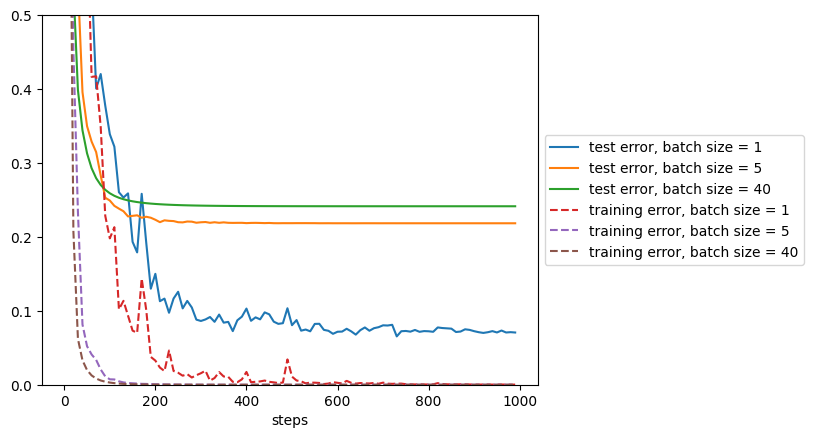
\includegraphics[width = 15cm]{implicitreg/implicitreg_quadratic_batchsize.png}
\end{figure}
Compared to the same initialization as in (f), the test error is significantly less for batch size 1, batch size 5 has some improvement, but batch size 40 performs just as bad as the standard GD. This shows that SGD can improve model generalization significantly.
\end{answer}
	}\fi
\end{enumerate}
